\documentclass[12pt]{article}

% defining image path
\usepackage{graphicx}
\graphicspath{ {./images/} }

% tables
\usepackage[utf8]{inputenc}
\usepackage[table]{xcolor}
\usepackage{enumitem}
\usepackage{multirow}
%\usepackage{multicol}
% \usepackage{adjustbox}
% \usepackage{tabularx}
% \newcolumntype{L}{>{\raggedright\arraybackslash}X}

\setlist{nolistsep}

\pagestyle{empty}
\setcounter{secnumdepth}{2}


\topmargin=0cm
\oddsidemargin=0cm
\textheight=22.0cm
\textwidth=16cm 

\parindent=0cm
\parskip=0.15cm
\topskip=0truecm
\raggedbottom
\abovedisplayskip=3mm
\belowdisplayskip=3mm
\abovedisplayshortskip=0mm
\belowdisplayshortskip=2mm
\normalbaselineskip=12pt
\normalbaselines

\begin{document}
\vspace*{0.5in}
\centerline{\bf\Large
Requirements for the Kakuro project}


\vspace*{0.5in}
\centerline{\bf\Large Iteration 2 COMP354}

\vspace*{0.5in}
\centerline{\bf\Large Team PK-A}

\vspace*{0.5in}
\centerline{\bf\Large 15 March 2020}

\vspace*{1.5in}
\begin{table}[htbp]
\caption{Team Members}
\begin{center}
\begin{tabular}{|c |c | c|}
\hline
Name & Role & ID Number \\
\hline\hline
Tiffany Ah King & Quality Control & 40082976 \\
\hline
Isabelle Charette & Documenter & 40008121 \\
\hline
Brian Gamboc-Javiniar & Coder & 40033124 \\
\hline
Vsevolod Ivanov & Organizer & 40004286 \\
\hline
Chang Liu & Quality Control & 40056360 \\
\hline
Nolan Mckay & Coder & 27873557 \\
\hline
Nalveer Moocheet & Quality Control & 40072605 \\
\hline
Hoang Thuan Pham & Coder & 40022992 \\
\hline
Audrey-Laure St-Louis & Documenter & 27558783 \\
\hline
Jia Ming Wei & Documenter & 40078192 \\
\hline
\end{tabular}
\end{center}
\end{table}


\newpage

\renewcommand*\contentsname{Table of Contents}

\tableofcontents

\clearpage

\section{Introduction}

\subsubsection{Purpose}
The purpose of this document is to present the design of the Kakuro game for the course COMP 354. 

\subsubsection{Scope}
This document is intended to provide detailed design specifications of the Kakuro game.

\newpage

\section{Architectural Design} \label{sec:arch}



\subsection{Architectural Diagram}

\begin{figure}[htbp]
    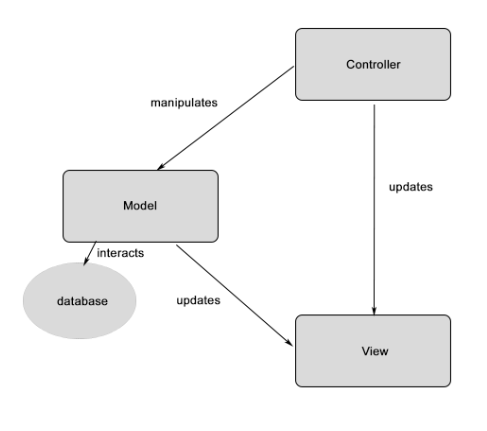
\includegraphics[width=0.7\textwidth]{archi_diagram}
    \caption{Architecture Diagram}
    \label{fig:archi_diagram}
\end{figure}

\subsubsection{Rationale}

The architecture chosen for the Kakuro game is the Model View Controller model (MVC). The MVC architecture is constructed of three separate components: the model, the view and the controller.

The model is the central component of the game. It stores the data and it changes depending on the state of the game. In Kakuro, the model stores the information of the cells from the rows and the columns displayed by the graphical user interface. The view is the graphical user interface (GUI) of the game. It displays the grid, the buttons, and the text elements but it also displays the date from the model. It allows the player to enter numbers to play the game. Whenever the model changes, the GUI reacts to these changes by updating itself. For example, if the player presses the button restart, the model will be updated by clearing its input cells and therefore, the GUI will react by showing empty input cells to the user.

The controller manages the interactions with the user and decides which functions should be called given an action. The controller will use the model’s data, he will take action on those depending on the user’s action and he will send it to the view for it to show it in the GUI.


\subsection{Subsystem Interface Specifications}

Specification of the software interfaces between the subsystems,
i.e. specific messages (or function calls) that are exchanged by the subsystems.
These are also often called ``Module Interface Specifications''.
Description of the parameters to be passed into these function calls in order to have a service fulfilled,
including valid and invalid ranges of values.
Each subsystem interface must be presented in a separate subsection.

\newpage

\section{Detailed Design} \label{sec:detail}

The Karuro system consists of three subsystems: Game-Puzzle, Registration, and Ranking subsystems. The Game-Puzzle subsystem is implemented in the iteration 1 and iteration 2. During the iteration 1, this subsystem is implemented using the UI and the console. During the iteration 2, a SQLite server is integrated in the libraries so that the input data and solution data are possible to be stored in the database. Therefore, having a database server is essential to implement the Registration subsystem and Ranking subsystem in the iteration 3. 

\begin{figure}[htbp]
    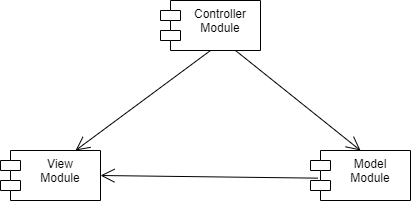
\includegraphics[width=1\textwidth]{Subsystems_UML}
    \caption{UML of Kakuro Subsystems}
    \label{fig:Subsystems_UML}
\end{figure}

The three subsystem are derived from the whole system, the Karuro system. On the other hand, the three subsystems are independent of each other. This design practice the principles of high cohesion and low coupling. The three subsystems are also three components of this software systems. The three subsystems present three different views, apply different models, and use different controller. The Ranking subsystem intersects with the Registration subsystem in the username-score part, and both of them have dependency with the Game-Puzzle subsystem in the aspect of game score coming from the game result and the specific user of that game.

% Complete description of the system design, describing one subsystem separately in respective subsection.
% UML class diagrams are to be used, as well as a short textual description describing the purpose of each class.


\newpage

\subsection{Game-Puzzle Subsystem}

\subsubsection{Detailed Design Diagram}

\begin{figure}[htbp]
    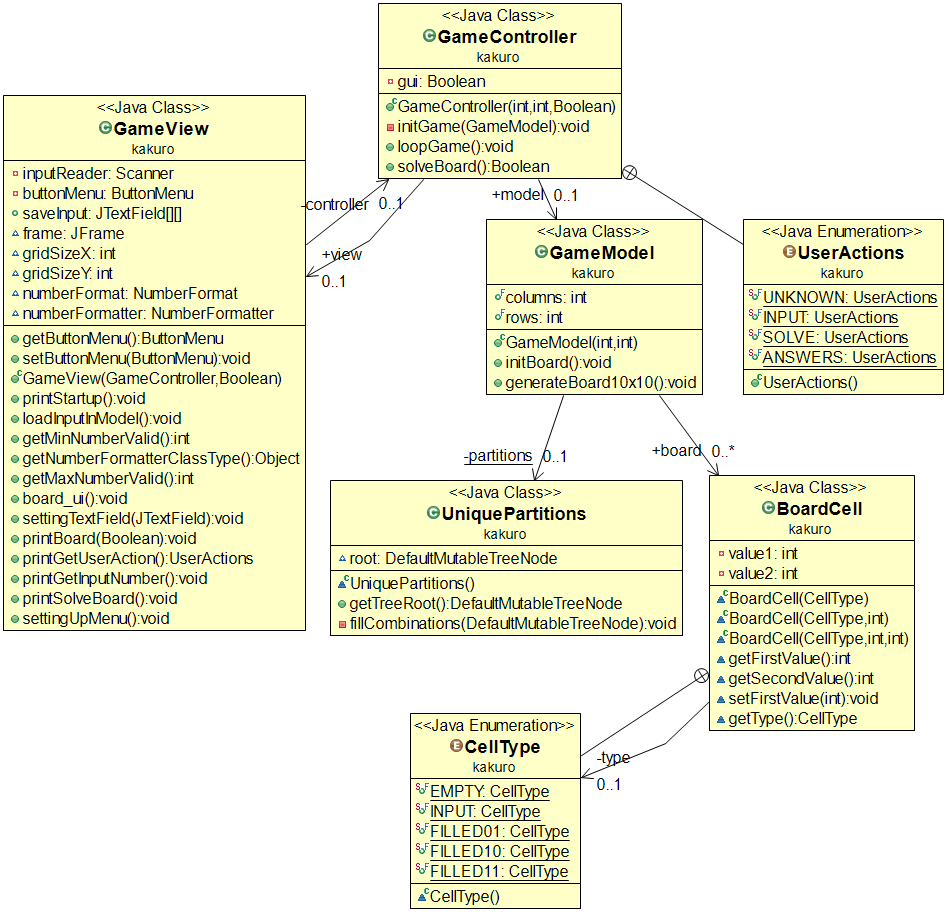
\includegraphics[width=1\textwidth]{GamePuzzle_UML}
    \caption{UML of Geme-Puzzle Subsystems}
    \label{fig:GamePuzzle_UML}
\end{figure}



\newpage

\subsubsection{Units Description}

List each class in this subsystem and write a short description of its purpose,
as well as notes or reminders useful for the programmers who will implement them.
List all attributes and functions of the class.


\begin{flushleft}
\begin{tabular}{| l | l | l | l | l |}
    \hline
    \textbf{Class Name} & \multicolumn{4}{ l |} {\textbf{GameController}} \\
    \hline
    Inherits from & \multicolumn{4}{ l |}{None} \\
    \hline
    Description & \multicolumn{4}{ l |} {The controller of subsystem} \\
    \hline
    \multirow{3}{*}{Attributes} & Visibility & Data Type & Name & Description \\\cline{2-5}
     & Public & enum & UserActions & User actions \\\cline{2-5}
     & Private & Boolean & gui & GUI or console \\
    \hline
    \multirow{5}{*}{Methods} & Visibility & Method Name & \multicolumn{2}{l |}{Description} \\\cline{2-5}
    
    & Public & GameController(int, int, Boolean) & \multicolumn{2}{l |}{Constructor} \\
    \cline{2-5}
    & Public & loopGame() & \multicolumn{2}{l |}{A loop that keep game running} \\
    \cline{2-5}
    & Public & solveBoard() & \multicolumn{2}{l |}{To check if the answer is correct } \\
    \cline{2-5}
    & Private & initGame(GameModel) & \multicolumn{2}{l |}{To initiate a new game} \\
    \hline
\end{tabular}
\end{flushleft}

\begin{flushleft}
\begin{tabular}{| l | l | l | l | l |}
    \hline
    \textbf{Class Name} & \multicolumn{4}{ l |} {\textbf{GameModel}} \\
    \hline
    Inherits from & \multicolumn{4}{ l |}{None} \\
    \hline
    Description & \multicolumn{4}{ l |} {The view of subsystem} \\
    \hline
    \multirow{3}{*}{Attributes} & Visibility & Data Type & Name & Description \\
    \cline{2-5}
    
     & Public & int & columns & The columns of the board \\
    \cline{2-5}
    & Public & int & rows & The rows of the board \\
    \hline
    \multirow{4}{*}{Methods} & Visibility & Method Name & \multicolumn{2}{l |}{Description} \\
    \cline{2-5}
    & Public & GameModel(int, int) & \multicolumn{2}{l |}{Constructor} \\
    \cline{2-5}
    & Public & initBoard() & \multicolumn{2}{l |}{To initiate a new board} \\
    \cline{2-5}
    & Public & generateBoard10x10() & \multicolumn{2}{l |}{To generate a 10x10 board} \\
    \hline
\end{tabular}
\end{flushleft}

\newpage
\begin{flushleft}
\begin{tabular}{| p{2cm} | l | l | l | p{58.8mm} |}

    \hline
    \textbf{Class Name} & \multicolumn{4}{ l |} {\textbf{GameView}} \\
    \hline
    Inherits from & \multicolumn{4}{ l |}{None} \\
    \hline
    Description & \multicolumn{4}{ l |} {The view of the subsystem} \\
    \hline
    \multirow{9}{*}{Attributes} & Visibility & Data Type & Name & Description \\
    \cline{2-5}
     & Private & Scanner & inputReader &  A input reader \\\cline{2-5}
     & Private & ButtonMenu & buttonMenu & A ButtonMenu object \\ \cline{2-5}
     & Private & JFrame & frame & A JFrame object \\ \cline{2-5}
     & Public & JTextField[][] & saveInput & The inputs array\\ \cline{2-5}
     & Private & int & gridSizeX & X value of grid size \\ \cline{2-5}
     & Private & int & gridSizeY & Y value of grid size \\ \cline{2-5}
     & Private & NumberFormat & numberFormat & A number format instance \\ \cline{2-5}
     & Private & NumberFormatter & numberFormatter & A NumberFormatter instance \\ 
    \hline
    \end{tabular}
    \begin{tabular}{| p{2cm} | l | l | l | p{5cm} |}
    \multirow{16}{*}{Methods} & Visibility & Method Name & \multicolumn{2}{l |}{Description} \\
    \cline{2-5}
    & Public & GameView(GameController, Boolean) &  \multicolumn{2}{l |}{Constructor} \\\cline{2-5}
    & Public & getButtonMenu() & \multicolumn{2}{l |}{Return a ButtonMenu object} \\\cline{2-5}
    & Public & setButtonMenu() & \multicolumn{2}{l |}{Set a value} \\\cline{2-5}
    & Public & printStartup() & \multicolumn{2}{l |}{Displays instructions in console} \\\cline{2-5}
    & Public & loadInputInModel() & \multicolumn{2}{l |}{To load input model} \\\cline{2-5}
    & Public & getMinNumberValid() & \multicolumn{2}{l |}{Return a minimum valid integer} \\\cline{2-5}
    & Public & getMaxNumberValid() & \multicolumn{2}{l |}{Return a maximum valid integer} \\\cline{2-5}
    & Public & getNumberFormatterClassType() & \multicolumn{2}{l |}{Return a class type} \\\cline{2-5}
    & Public & boardUi() & \multicolumn{2}{l |}{To create an user interface} \\\cline{2-5}
    & Public & settingTextField(JTextField) & \multicolumn{2}{l |}{To set the text fields of board} \\\cline{2-5}
    & Public & settingUpMenu() & \multicolumn{2}{l |}{To set up the button menu} \\\cline{2-5}
    & Public & printBoard(Boolean) & \multicolumn{2}{l |}{Displays input in console} \\\cline{2-5}
    & Public & printGetUserAction() & \multicolumn{2}{l |}{Reads user actions from console} \\\cline{2-5}
    & Public & printGetInputNumber() & \multicolumn{2}{l |}{Displays and validates inputs} \\\cline{2-5}
    & Public & printSolveBoard() & \multicolumn{2}{l |}{Displays the solution correctness} \\
    \hline
\end{tabular}
\end{flushleft}

\begin{flushleft}
\begin{tabular}{| l | l | l | l | l |}
    \hline
    \textbf{Class Name} & \multicolumn{4}{ l |} {\textbf{UniquePartitions}} \\
    \hline
    Inherits from & \multicolumn{4}{ l |}{None} \\
    \hline
    Description & \multicolumn{4}{ l |} {Lists all possible answers in a Tree ADT} \\
    \hline
    \multirow{2}{*}{Attributes} & Visibility & Data Type & Name & Description \\
    \cline{2-5}
     & Private & DefaultMutableTreeNode & root & A root node object \\
    \hline
    \multirow{4}{*}{Methods} & Visibility & Method Name & \multicolumn{2}{l |}{Description} \\
    \cline{2-5}
    & Public & UniquePartitions() & \multicolumn{2}{l |}{Constructor} \\
    \cline{2-5}
    & Public & getTreeRoot() & \multicolumn{2}{l |}{Returns a root node object} \\
    \cline{2-5}
    & Public & fillCombinations(DefaultMutableTreeNode) & \multicolumn{2}{p{5cm} |}{Fills cells with possible number combinations to solve the puzzle}\\
    \hline
\end{tabular}
\end{flushleft}

% \begin{flushleft}
% \begin{tabular}{| l | l | l | l | l |}
%     \hline
%     \textbf{Class Name} & \multicolumn{4}{ l |} {\textbf{}} \\
%     \hline
%     Inherits from & \multicolumn{4}{ l |}{None} \\
%     \hline
%     Description & \multicolumn{4}{ l |} {} \\
%     \hline
%     \multirow{2}{*}{Attributes} & Visibility & Data Type & Name & Description \\
%     \cline{2-5}
%      & Private &  &  &  \\
%     \hline
%     \multirow{2}{*}{Methods} & Visibility & Method Name & \multicolumn{2}{l |}{Description} \\
%     \cline{2-5}
%     & Public &  & \multicolumn{2}{l |}{} \\
%     \hline
% \end{tabular}
% \end{flushleft}

\begin{flushleft}
\begin{tabular}{| l | l | l | l | l |}
    \hline
    \textbf{Class Name} & \multicolumn{4}{ l |} {\textbf{BoardCell}} \\
    \hline
    Inherits from & \multicolumn{4}{ l |}{None} \\
    \hline
    Description & \multicolumn{4}{ l |} {A cell of game board} \\
    \hline
    \multirow{4}{*}{Attributes} & Visibility & Data Type & Name & Description \\
    \cline{2-5}
     & Private & int & value1 & A value of cell \\
     \cline{2-5}
     & Private & int & value2 & A value of cell \\
     \cline{2-5}
     & Package & enum & CellType & Five cell types in game board \\
    \hline
    \multirow{8}{*}{Methods} & Visibility & Method Name & \multicolumn{2}{l |}{Description} \\
    \cline{2-5}
    & Public & BoardCell(CellType) & \multicolumn{2}{l |}{Constructor} \\
    \cline{2-5}
    & Public & BoardCell(CellType, int) & \multicolumn{2}{l |}{Constructor} \\
    \cline{2-5}
    & Public & BoardCell(CellType, int, int) & \multicolumn{2}{l |}{Constructor} \\
    \cline{2-5}
    & Public & getFirstValue() & \multicolumn{2}{l |}{Returns value1} \\
    \cline{2-5}
    & Public & getSecondValue() & \multicolumn{2}{l |}{Returns value2} \\
    \cline{2-5}
    & Public & setFirstValue(int) & \multicolumn{2}{l |}{Sets value1} \\
    \cline{2-5}
    & Public & getType() & \multicolumn{2}{l |}{Retutns a cell type} \\
    \hline
\end{tabular}
\end{flushleft}

% \begin{flushleft}
% \begin{tabular}{| l | l | l | l | l |}
%     \hline
%     \textbf{Class Name} & \multicolumn{4}{ l |} {\textbf{}} \\
%     \hline
%     Inherits from & \multicolumn{4}{ l |}{None} \\
%     \hline
%     Description & \multicolumn{4}{ l |} {} \\
%     \hline
%     Attributes & Visibility & Data Type & Name & Description \\
%     \hline
%      & Private &  &  &  \\
%     \hline
%     Methods & Visibility & Method Name & \multicolumn{2}{l |}{Description} \\
%     \hline
%     & Public &  & \multicolumn{2}{l |}{} \\
%     \hline
% \end{tabular}
% \end{flushleft}

% \begin{center}
% \setlength{\tabcolsep}{18pt}
% \renewcommand{\arraystretch}{1.1}
% \begin{tabular}{ |p{3.4cm}|p{10cm}| }
%     \hline
%     \textbf{Method Name} & \textbf{} \\
%     \hline
%     Class Name &  \\
%     \hline
%     Functionality &  \\
%     \hline
%     Input & None \\
%     \hline
%     Output & None \\
%     \hline
%     Pseudo Code &  
%     \vspace*{-0.1in}
%     \begin{enumerate}[leftmargin=0.2in]
%     \item The application is running
%     \item No game is in progress
%     \end{enumerate}  \\
%     \hline
% \end{tabular}
% \end{center}

\newpage

\subsection{Registration Subsystem}

\subsubsection{Detailed Design Diagram}

UML class diagram depicting the internal structure of the subsystem,
accompanied by a paragraph of text describing the rationale of this design.

\subsubsection{Units Description}

List each class in this subsystem and write a short description of its purpose,
as well as notes or reminders useful for the programmers who will implement them.
List all attributes and functions of the class.

\newpage

\subsection{Ranking Subsystem}

\subsubsection{Detailed Design Diagram}

UML class diagram depicting the internal structure of the subsystem,
accompanied by a paragraph of text describing the rationale of this design.

\subsubsection{Units Description}

List each class in this subsystem and write a short description of its purpose,
as well as notes or reminders useful for the programmers who will implement them.
List all attributes and functions of the class.

\newpage

\section{Dynamic Design Scenarios}
The following are the descriptions of the execution scenarios of the game initialization, the process of saving a game and the process of loading a game. These systems are involved in the subsystem of the puzzle mechanics.



\subsection{Initialize Game (UI only)}
\begin{figure}[htbp]
    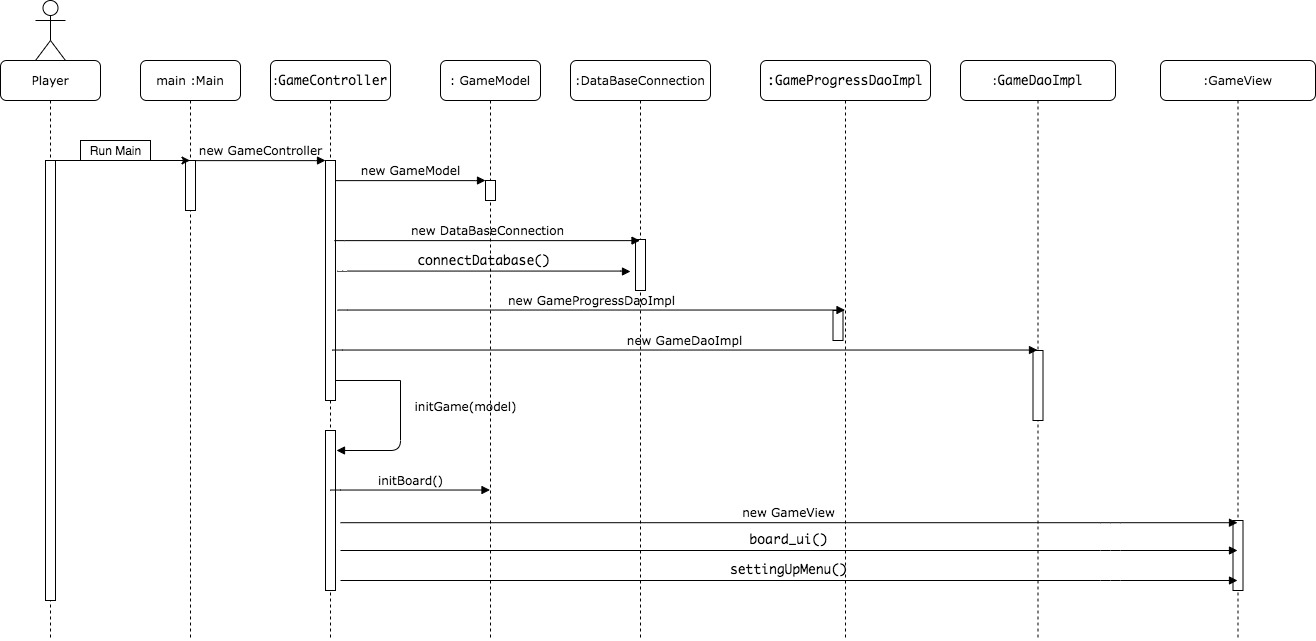
\includegraphics[width=1\textwidth]{initializeGame_UI}
    \caption{Sequence diagram to initialize a game}
    \label{fig:sequenceDiagram}
\end{figure}

\newpage

\subsection{Save Game}
\begin{figure}[htbp]
    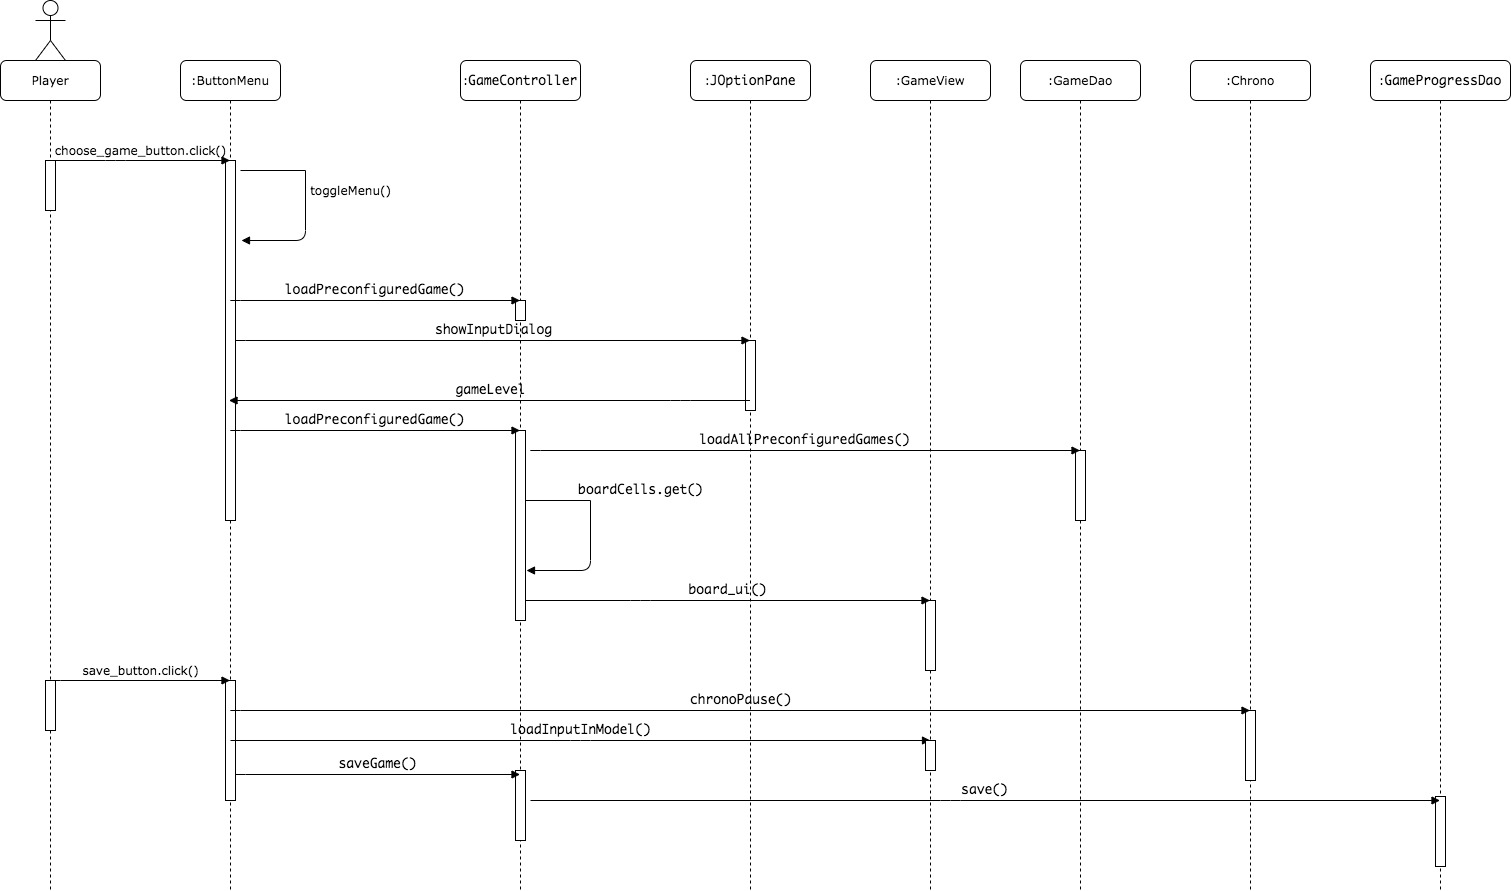
\includegraphics[width=1\textwidth]{saveGame}
    \caption{Sequence diagram to save a game}
    \label{fig:sequenceDiagram}
\end{figure}

\newpage

\subsection{Load Game}
\begin{figure}[htbp]
    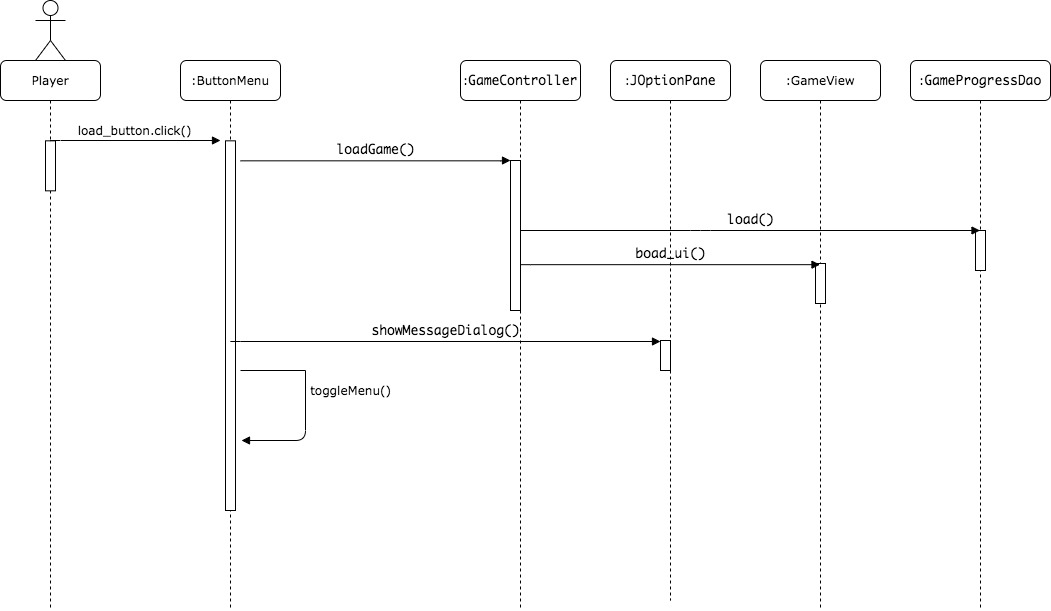
\includegraphics[width=1\textwidth]{loadGame}
    \caption{Sequence diagram to load a game}
    \label{fig:sequenceDiagram}
\end{figure}
\end{document}
